\documentclass[11pt,addpoints,answers]{exam}

%-----------------------------------------------------------------------------
% PACKAGES AND OTHER DOCUMENT CONFIGURATIONS
%-----------------------------------------------------------------------------

\usepackage[margin=1in]{geometry}
\usepackage{amsmath, amsfonts}
\usepackage{enumerate}
\usepackage{graphicx}
\usepackage{titling}
\usepackage{url}
\usepackage{xfrac}
\usepackage{natbib}
\usepackage{amssymb}
\usepackage{amsthm}
\usepackage{paralist}
\usepackage{epstopdf}
\usepackage{tabularx}
\usepackage{longtable}
\usepackage{multirow}
\usepackage{multicol}
\usepackage[colorlinks=true,urlcolor=blue]{hyperref}
\usepackage{algorithm}
\usepackage{algorithmicx}
\usepackage[noend]{algpseudocode}
\usepackage{float}
\usepackage{enumerate}
\usepackage{array}
\usepackage{environ}
\usepackage{times}
\usepackage{textcomp}
\usepackage{caption}
\usepackage{parskip} % For NIPS style paragraphs.
\usepackage[compact]{titlesec} % Less whitespace around titles
\usepackage[inline]{enumitem} % For inline enumerate* and itemize*
\usepackage{datetime}
\usepackage{comment}
% \usepackage{minted}
\usepackage{lastpage}
\usepackage{color}
\usepackage{xcolor}
\usepackage[final]{listings}
\usepackage{tikz}
\usetikzlibrary{shapes,decorations, arrows}
\usepackage{framed}
\usepackage{booktabs}
\usepackage{cprotect}
\usepackage{verbatimbox}
\usepackage{multicol}
\usepackage{hyperref}
\usepackage{subcaption}
\usepackage{mathtools} % For drcases
\usepackage{cancel}
\usepackage[many]{tcolorbox}
\usepackage{soul}
\usepackage[bottom]{footmisc}
\usepackage{bm}
\usepackage{wasysym}

\usepackage{tikz}
\usetikzlibrary{arrows}
\usetikzlibrary{arrows.meta}
\usetikzlibrary{shapes.geometric}
\usetikzlibrary{positioning, arrows, automata, calc}

\newtcolorbox[]{your_solution}[1][]{
    % breakable,
    enhanced,
    nobeforeafter,
    colback=white,
    title=Your Answer,
    sidebyside align=top,
    box align=top,
    #1
}

%%%%%%%%%%%%%%%%%%%%%%%%%%%%%%%%%%%%%%%%%%%
% Formatting for \CorrectChoice of "exam" %
%%%%%%%%%%%%%%%%%%%%%%%%%%%%%%%%%%%%%%%%%%%

\CorrectChoiceEmphasis{}
\checkedchar{\blackcircle}

%%%%%%%%%%%%%%%%%%%%%%%%%%%%%%%%%%%%%%%%%%%
% Rotated Column Headers                  %
%%%%%%%%%%%%%%%%%%%%%%%%%%%%%%%%%%%%%%%%%%%
\usepackage{adjustbox}
\usepackage{array}

%https://tex.stackexchange.com/questions/32683/rotated-column-titles-in-tabular

\newcolumntype{R}[2]{%
    >{\adjustbox{angle=#1,lap=\width-(#2)}\bgroup}%
    l%
    <{\egroup}%
}
\newcommand*\rot{\multicolumn{1}{R{45}{1em}}}% no optional argument here, please!

%%%%%%%%%%%%%%%%%%%%%%%%%%%%%%%%%%%%%%%%%%
% Custom commands                        %
%%%%%%%%%%%%%%%%%%%%%%%%%%%%%%%%%%%%%%%%%%

\newcommand{\vc}[1]{\boldsymbol{#1}}
\newcommand{\adj}[1]{\frac{d J}{d #1}}
\newcommand{\chain}[2]{\adj{#2} = \adj{#1}\frac{d #1}{d #2}}

\newcommand{\R}{\mathbb{R}}
\newcommand{\blackcircle}{\tikz\draw[black,fill=black] (0,0) circle (1ex);}
\renewcommand{\circle}{\tikz\draw[black] (0,0) circle (1ex);}

\newcommand{\emptysquare}{{\LARGE $\square$}\ \ }
\newcommand{\filledsquare}{{\LARGE $\boxtimes$}\ \ }
\newcommand{\emptycircle}{{\LARGE $\fullmoon$}\ \ }
\newcommand{\filledcircle}{{\LARGE $\newmoon$}\ \ }

\newcommand{\ntset}{test}

% mathcal
\newcommand{\Ac}{\mathcal{A}}
\newcommand{\Bc}{\mathcal{B}}
\newcommand{\Cc}{\mathcal{C}}
\newcommand{\Dc}{\mathcal{D}}
\newcommand{\Ec}{\mathcal{E}}
\newcommand{\Fc}{\mathcal{F}}
\newcommand{\Gc}{\mathcal{G}}
\newcommand{\Hc}{\mathcal{H}}
\newcommand{\Ic}{\mathcal{I}}
\newcommand{\Jc}{\mathcal{J}}
\newcommand{\Kc}{\mathcal{K}}
\newcommand{\Lc}{\mathcal{L}}
\newcommand{\Mc}{\mathcal{M}}
\newcommand{\Nc}{\mathcal{N}}
\newcommand{\Oc}{\mathcal{O}}
\newcommand{\Pc}{\mathcal{P}}
\newcommand{\Qc}{\mathcal{Q}}
\newcommand{\Rc}{\mathcal{R}}
\newcommand{\Sc}{\mathcal{S}}
\newcommand{\Tc}{\mathcal{T}}
\newcommand{\Uc}{\mathcal{U}}
\newcommand{\Vc}{\mathcal{V}}
\newcommand{\Wc}{\mathcal{W}}
\newcommand{\Xc}{\mathcal{X}}
\newcommand{\Yc}{\mathcal{Y}}
\newcommand{\Zc}{\mathcal{Z}}

% mathbb
\newcommand{\Ab}{\mathbb{A}}
\newcommand{\Bb}{\mathbb{B}}
\newcommand{\Cb}{\mathbb{C}}
\newcommand{\Db}{\mathbb{D}}
\newcommand{\Eb}{\mathbb{E}}
\newcommand{\Fb}{\mathbb{F}}
\newcommand{\Gb}{\mathbb{G}}
\newcommand{\Hb}{\mathbb{H}}
\newcommand{\Ib}{\mathbb{I}}
\newcommand{\Jb}{\mathbb{J}}
\newcommand{\Kb}{\mathbb{K}}
\newcommand{\Lb}{\mathbb{L}}
\newcommand{\Mb}{\mathbb{M}}
\newcommand{\Nb}{\mathbb{N}}
\newcommand{\Ob}{\mathbb{O}}
\newcommand{\Pb}{\mathbb{P}}
\newcommand{\Qb}{\mathbb{Q}}
\newcommand{\Rb}{\mathbb{R}}
\newcommand{\Sb}{\mathbb{S}}
\newcommand{\Tb}{\mathbb{T}}
\newcommand{\Ub}{\mathbb{U}}
\newcommand{\Vb}{\mathbb{V}}
\newcommand{\Wb}{\mathbb{W}}
\newcommand{\Xb}{\mathbb{X}}
\newcommand{\Yb}{\mathbb{Y}}
\newcommand{\Zb}{\mathbb{Z}}

% mathbf lowercase
\newcommand{\av}{\mathbf{a}}
\newcommand{\bv}{\mathbf{b}}
\newcommand{\cv}{\mathbf{c}}
\newcommand{\dv}{\mathbf{d}}
\newcommand{\ev}{\mathbf{e}}
\newcommand{\fv}{\mathbf{f}}
\newcommand{\gv}{\mathbf{g}}
\newcommand{\hv}{\mathbf{h}}
\newcommand{\iv}{\mathbf{i}}
\newcommand{\jv}{\mathbf{j}}
\newcommand{\kv}{\mathbf{k}}
\newcommand{\lv}{\mathbf{l}}
\newcommand{\mv}{\mathbf{m}}
\newcommand{\nv}{\mathbf{n}}
\newcommand{\ov}{\mathbf{o}}
\newcommand{\pv}{\mathbf{p}}
\newcommand{\qv}{\mathbf{q}}
\newcommand{\rv}{\mathbf{r}}
\newcommand{\sv}{\mathbf{s}}
\newcommand{\tv}{\mathbf{t}}
\newcommand{\uv}{\mathbf{u}}
\newcommand{\vv}{\mathbf{v}}
\newcommand{\wv}{\mathbf{w}}
\newcommand{\xv}{\mathbf{x}}
\newcommand{\yv}{\mathbf{y}}
\newcommand{\zv}{\mathbf{z}}

% mathbf uppercase
\newcommand{\Av}{\mathbf{A}}
\newcommand{\Bv}{\mathbf{B}}
\newcommand{\Cv}{\mathbf{C}}
\newcommand{\Dv}{\mathbf{D}}
\newcommand{\Ev}{\mathbf{E}}
\newcommand{\Fv}{\mathbf{F}}
\newcommand{\Gv}{\mathbf{G}}
\newcommand{\Hv}{\mathbf{H}}
\newcommand{\Iv}{\mathbf{I}}
\newcommand{\Jv}{\mathbf{J}}
\newcommand{\Kv}{\mathbf{K}}
\newcommand{\Lv}{\mathbf{L}}
\newcommand{\Mv}{\mathbf{M}}
\newcommand{\Nv}{\mathbf{N}}
\newcommand{\Ov}{\mathbf{O}}
\newcommand{\Pv}{\mathbf{P}}
\newcommand{\Qv}{\mathbf{Q}}
\newcommand{\Rv}{\mathbf{R}}
\newcommand{\Sv}{\mathbf{S}}
\newcommand{\Tv}{\mathbf{T}}
\newcommand{\Uv}{\mathbf{U}}
\newcommand{\Vv}{\mathbf{V}}
\newcommand{\Wv}{\mathbf{W}}
\newcommand{\Xv}{\mathbf{X}}
\newcommand{\Yv}{\mathbf{Y}}
\newcommand{\Zv}{\mathbf{Z}}

% bold greek lowercase
\newcommand{\alphav     }{\boldsymbol \alpha     }
\newcommand{\betav      }{\boldsymbol \beta      }
\newcommand{\gammav     }{\boldsymbol \gamma     }
\newcommand{\deltav     }{\boldsymbol \delta     }
\newcommand{\epsilonv   }{\boldsymbol \epsilon   }
\newcommand{\varepsilonv}{\boldsymbol \varepsilon}
\newcommand{\zetav      }{\boldsymbol \zeta      }
\newcommand{\etav       }{\boldsymbol \eta       }
\newcommand{\thetav     }{\boldsymbol \theta     }
\newcommand{\varthetav  }{\boldsymbol \vartheta  }
\newcommand{\iotav      }{\boldsymbol \iota      }
\newcommand{\kappav     }{\boldsymbol \kappa     }
\newcommand{\varkappav  }{\boldsymbol \varkappa  }
\newcommand{\lambdav    }{\boldsymbol \lambda    }
\newcommand{\muv        }{\boldsymbol \mu        }
\newcommand{\nuv        }{\boldsymbol \nu        }
\newcommand{\xiv        }{\boldsymbol \xi        }
\newcommand{\omicronv   }{\boldsymbol \omicron   }
\newcommand{\piv        }{\boldsymbol \pi        }
\newcommand{\varpiv     }{\boldsymbol \varpi     }
\newcommand{\rhov       }{\boldsymbol \rho       }
\newcommand{\varrhov    }{\boldsymbol \varrho    }
\newcommand{\sigmav     }{\boldsymbol \sigma     }
\newcommand{\varsigmav  }{\boldsymbol \varsigma  }
\newcommand{\tauv       }{\boldsymbol \tau       }
\newcommand{\upsilonv   }{\boldsymbol \upsilon   }
\newcommand{\phiv       }{\boldsymbol \phi       }
\newcommand{\varphiv    }{\boldsymbol \varphi    }
\newcommand{\chiv       }{\boldsymbol \chi       }
\newcommand{\psiv       }{\boldsymbol \psi       }
\newcommand{\omegav     }{\boldsymbol \omega     }

% bold greek uppercase
\newcommand{\Gammav     }{\boldsymbol \Gamma     }
\newcommand{\Deltav     }{\boldsymbol \Delta     }
\newcommand{\Thetav     }{\boldsymbol \Theta     }
\newcommand{\Lambdav    }{\boldsymbol \Lambda    }
\newcommand{\Xiv        }{\boldsymbol \Xi        }
\newcommand{\Piv        }{\boldsymbol \Pi        }
\newcommand{\Sigmav     }{\boldsymbol \Sigma     }
\newcommand{\Upsilonv   }{\boldsymbol \Upsilon   }
\newcommand{\Phiv       }{\boldsymbol \Phi       }
\newcommand{\Psiv       }{\boldsymbol \Psi       }
\newcommand{\Omegav     }{\boldsymbol \Omega     }

%%%%%%%%%%%%%%%%%%%%%%%%%%%%%%%%%%%%%%%%%%%
% Code highlighting with listings         %
%%%%%%%%%%%%%%%%%%%%%%%%%%%%%%%%%%%%%%%%%%%

\definecolor{bluekeywords}{rgb}{0.13,0.13,1}
\definecolor{greencomments}{rgb}{0,0.5,0}
\definecolor{redstrings}{rgb}{0.9,0,0}
\definecolor{light-gray}{gray}{0.95}

\newcommand{\MYhref}[3][blue]{\href{#2}{\color{#1}{#3}}}%

\definecolor{dkgreen}{rgb}{0,0.6,0}
\definecolor{gray}{rgb}{0.5,0.5,0.5}
\definecolor{mauve}{rgb}{0.58,0,0.82}

\lstdefinelanguage{Shell}{
  keywords={tar, cd, make},
  %keywordstyle=\color{bluekeywords}\bfseries,
  alsoletter={+},
  ndkeywords={python, py, javac, java, gcc, c, g++, cpp, .txt, octave, m, .tar},
  %ndkeywordstyle=\color{bluekeywords}\bfseries,
  identifierstyle=\color{black},
  sensitive=false,
  comment=[l]{//},
  morecomment=[s]{/*}{*/},
  commentstyle=\color{purple}\ttfamily,
  %stringstyle=\color{red}\ttfamily,
  morestring=[b]',
  morestring=[b]",
  backgroundcolor = \color{light-gray}
}

\lstset{columns=fixed, basicstyle=\ttfamily,
    backgroundcolor=\color{light-gray},xleftmargin=0.5cm,frame=tlbr,framesep=4pt,framerule=0pt}


%%%%%%%%%%%%%%%%%%%%%%%%%%%%%%%%%%%%%%%%%%%
% Custom box for highlights               %
%%%%%%%%%%%%%%%%%%%%%%%%%%%%%%%%%%%%%%%%%%%

% Define box and box title style
\tikzstyle{mybox} = [fill=blue!10, very thick,
    rectangle, rounded corners, inner sep=1em, inner ysep=1em]

% \newcommand{\notebox}[1]{
% \begin{tikzpicture}
% \node [mybox] (box){%
%     \begin{minipage}{\textwidth}
%     #1
%     \end{minipage}
% };
% \end{tikzpicture}%
% }

\NewEnviron{notebox}{

\begin{tikzpicture}
\node [mybox] (box){
    \begin{minipage}{\textwidth}
        \BODY
    \end{minipage}
};
\end{tikzpicture}
}

%%%%%%%%%%%%%%%%%%%%%%%%%%%%%%%%%%%%%%%%%%%
% Commands showing / hiding solutions     %
%%%%%%%%%%%%%%%%%%%%%%%%%%%%%%%%%%%%%%%%%%%

%% To HIDE SOLUTIONS (to post at the website for students), set this value to 0: 
\def\issoln{0}
% Some commands to allow solutions to be embedded in the assignment file.
\ifcsname issoln\endcsname \else \def\issoln{1} \fi
% Default to an empty solutions environ.
\NewEnviron{soln}{}{}
\if\issoln 1
% Otherwise, include solutions as below.
\RenewEnviron{soln}{
    \leavevmode\color{red}\ignorespaces
    % \textbf{Solution} \BODY
    \BODY
}{}
\fi

%% To HIDE TAGS set this value to 0:
\def\showtags{0}
%%%%%%%%%%%%%%%%
\ifcsname showtags\endcsname \else \def\showtags{1} \fi
% Default to an empty tags environ.
\NewEnviron{tags}{}{}
\if\showtags 1
% Otherwise, include solutions as below.
\RenewEnviron{tags}{
    \fbox{
    \leavevmode\color{blue}\ignorespaces
    \textbf{TAGS:} \texttt{\url{\BODY}}
    }
    \vspace{-.5em}
}{}
\fi

%%%%%%%%%%%%%%%%%%%%%%%%%%%%%%%%%%%%%%%%%%%
% Commands for customizing the assignment %
%%%%%%%%%%%%%%%%%%%%%%%%%%%%%%%%%%%%%%%%%%%

\newcommand{\courseName}{10-301/10-601 Introduction to Machine Learning (Spring 2021)}
\newcommand{\hwName}{Homework 9: Learning Paradigms}
\newcommand{\dueDate}{TODO}


\title{\textsc{\hwName}
%\thanks{Compiled on \today{} at \currenttime{}}
} % Title


\author{\courseName\\
\url{http://www.cs.cmu.edu/~mgormley/courses/10601/} \\
OUT:  2022-04-21 \\
DUE:  2022-04-27 \\ 
TAs: Abbey, Abhi, Alex, Neural, Shelly, Udai
}

\date{}

%%%%%%%%%%%%%%%%%%%%%%%%%%%%%%%%%%%%%%%%%%%%%%%%%
% Useful commands for typesetting the questions %
%%%%%%%%%%%%%%%%%%%%%%%%%%%%%%%%%%%%%%%%%%%%%%%%%

\newcommand \expect {\mathbb{E}}
\newcommand \mle [1]{{\hat #1}^{\rm MLE}}
\newcommand \map [1]{{\hat #1}^{\rm MAP}}
\newcommand \argmax {\operatorname*{argmax}}
\newcommand \argmin {\operatorname*{argmin}}
\newcommand \code [1]{{\tt #1}}
\newcommand \datacount [1]{\#\{#1\}}
\newcommand \ind [1]{\mathbb{I}\{#1\}}

%%%%%%%%%%%%%%%%%%%%%%%%%%
% Document configuration %
%%%%%%%%%%%%%%%%%%%%%%%%%%

% Don't display a date in the title and remove the white space
\predate{}
\postdate{}
\date{}

% Don't display an author and remove the white space
%\preauthor{}
%\postauthor{}

% Question type commands
\newcommand{\sall}{\textbf{Select all that apply: }}
\newcommand{\sone}{\textbf{Select one: }}
\newcommand{\tf}{\textbf{True or False: }}

% AdaBoost commands
\newcommand{\trainerr}[1]{\hat{\epsilon}_S \left(#1\right)}
\newcommand{\generr}[1]{\epsilon \left(#1\right)}
\newcommand{\D}{\mathcal{D}}
\newcommand{\margin}{\text{margin}}
\newcommand{\sign}{\text{sign}}
\newcommand{\PrS}{\hat{\Pr_{(x^{(i)}, y^{(i)}) \sim S}}}
\newcommand{\PrSinline}{\hat{\Pr}_{(x^{(i)}, y^{(i)}) \sim S}}  % inline PrS

% Abhi messing around with examdoc
\qformat{\textbf{{\Large \thequestion \; \; \thequestiontitle \ (\totalpoints \ points)}} \hfill}
\renewcommand{\thequestion}{\arabic{question}}
\renewcommand{\questionlabel}{\thequestion.}

\renewcommand{\thepartno}{\arabic{partno}}
\renewcommand{\partlabel}{\thepartno.}
\renewcommand{\partshook}{\setlength{\leftmargin}{0pt}}

\renewcommand{\thesubpart}{\alph{subpart}}
\renewcommand{\subpartlabel}{(\thesubpart)}

\renewcommand{\thesubsubpart}{\roman{subsubpart}}
\renewcommand{\subsubpartlabel}{\thesubsubpart.}

% copied from stack overflow, as all good things are
\newcommand\invisiblesection[1]{%
  \refstepcounter{section}%
  \addcontentsline{toc}{section}{\protect\numberline{\thesection}#1}%
  \sectionmark{#1}}

% quite possibly the worst workaround i have made for this class
\newcommand{\sectionquestion}[1]{
\titledquestion{#1}
\invisiblesection{#1}
~\vspace{-1em}
}

%%%%%%%%%%%%%%%%%%
% Begin Document %
%%%%%%%%%%%%%%%%%% 

\begin{document}

\maketitle

\begin{notebox}
This is the final homework assignment. This assignment covers \textbf{Graphical Models}, \textbf{Ensemble Methods}, \textbf{K-Means}, \textbf{PCA}, and \textbf{Recommender Systems}.
\end{notebox}
\newcommand \maxsubs {10 }
\section*{START HERE: Instructions}
\begin{itemize}

\item \textbf{Collaboration Policy}: Please read the collaboration policy here: \url{http://www.cs.cmu.edu/~mgormley/courses/10601/syllabus.html}

\item\textbf{Late Submission Policy:} See the late submission policy here: \url{http://www.cs.cmu.edu/~mgormley/courses/10601/syllabus.html}

\item\textbf{Submitting your work:} You will use Gradescope to submit
  answers to all questions and code. Please
  follow instructions at the end of this PDF to correctly submit all your code to Gradescope.

  \begin{itemize}
    
 % COMMENT IF NOT USING CANVAS
\begin{comment}
  \item \textbf{Canvas:} Canvas (\url{https://canvas.cmu.edu}) will be
    used for quiz-style problems (e.g. multiple choice, true / false,
    numerical answers). Grading is done automatically.
    %
    You may only \textbf{submit once} on canvas, so be sure of your
    answers before you submit. However, canvas allows you to work on
    your answers and then close out of the page and it will save your
    progress.  You will not be granted additional submissions, so
    please be confident of your solutions when you are submitting your
    assignment.
    %
    {\color{red} The above is true for future assignments, but this one
    allows {\bf unlimited submissions}.}
\end{comment}
    
  % COMMENT IF NOT USING GRADESCOPE
   \item \textbf{Written:} For written problems such as short answer, multiple choice, derivations, proofs, or plots, please use the provided template. Submissions can be handwritten onto the template, but should be labeled and clearly legible. If your writing is not legible, you will not be awarded marks. If your scanned submission misaligns the template, there will be a 5\% penalty. Alternatively, submissions can be written in LaTeX. 
   Each derivation/proof should be completed in the boxes provided. If you do not follow the template, your assignment may not be graded correctly by our AI assisted grader.
  \end{itemize}

\end{itemize}\clearpage

\section*{Instructions for Specific Problem Types}

For ``Select One" questions, please fill in the appropriate bubble completely:

\begin{quote}
\textbf{Select One:} Who taught this course?
    \begin{checkboxes}
     \CorrectChoice Matt Gormley
     \choice Marie Curie
     \choice Noam Chomsky
    \end{checkboxes}
\end{quote}

If you need to change your answer, you may cross out the previous answer and bubble in the new answer:

\begin{quote}
\textbf{Select One:} Who taught this course?
    {
    \begin{checkboxes}
     \CorrectChoice Matt Gormley
     \choice Marie Curie \checkboxchar{\xcancel{\blackcircle}{}}
     \choice Noam Chomsky
    \end{checkboxes}
    }
\end{quote}

For ``Select all that apply" questions, please fill in all appropriate squares completely:

\begin{quote}
\textbf{Select all that apply:} Which are scientists?
    {%
    \checkboxchar{$\Box$} \checkedchar{$\blacksquare$} % change checkbox style locally
    \begin{checkboxes}
    \CorrectChoice Stephen Hawking 
    \CorrectChoice Albert Einstein
    \CorrectChoice Isaac Newton
    \choice I don't know
    \end{checkboxes}
    }
\end{quote}

Again, if you need to change your answer, you may cross out the previous answer(s) and bubble in the new answer(s):

\begin{quote}
\textbf{Select all that apply:} Which are scientists?
    {%
    \checkboxchar{\xcancel{$\blacksquare$}} \checkedchar{$\blacksquare$} % change checkbox style locally
    \begin{checkboxes}
    \CorrectChoice Stephen Hawking 
    \CorrectChoice Albert Einstein
    \CorrectChoice Isaac Newton
    \choice I don't know
    \end{checkboxes}
    }
\end{quote}

For questions where you must fill in a blank, please make sure your final answer is fully included in the given space. You may cross out answers or parts of answers, but the final answer must still be within the given space.

\begin{quote}
\textbf{Fill in the blank:} What is the course number?

\begin{tcolorbox}[fit,height=1cm, width=4cm, blank, borderline={1pt}{-2pt},nobeforeafter]
    \begin{center}\huge10-601\end{center}
    \end{tcolorbox}\hspace{2cm}
    \begin{tcolorbox}[fit,height=1cm, width=4cm, blank, borderline={1pt}{-2pt},nobeforeafter]
    \begin{center}\huge10-\xcancel{6}301\end{center}
    \end{tcolorbox}
\end{quote}
\clearpage

{\LARGE \bf Written Questions (\numpoints \ points)}
\begin{questions}
\sectionquestion{\LaTeX{} Bonus Point}
\label{sec:latex}

\begin{parts}
    \part[1] \sone Did you use \LaTeX{} for the entire written portion of this homework?
    
    \begin{checkboxes}
        % YOUR ANSWER
        % Change \choice to \CorrectChoice for the appropriate selection/selections 
        \choice Yes
        \choice No
    \end{checkboxes}
\end{parts}\sectionquestion{Graphical Models}
\label{sec:bayes}

Consider the joint distribution over the binary random variables $A, B, C, D, E$ represented by the Bayesian Network shown in the figure.

\begin{center}
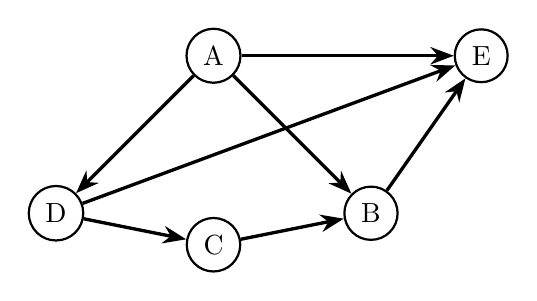
\begin{tikzpicture}
\begin{scope}[every node/.style={circle,thick,draw}]
    \node (A) at (0,0) {A};
    \node (B) at (2,-2) {B};
    \node (C) at (0,-2.4) {C};
    \node (D) at (-2,-2) {D};
    \node (E) at (3.4,0) {E};
\end{scope}

\begin{scope}[>={Stealth[black]},
              every node/.style={fill=white,circle},
              every edge/.style={draw=black,very thick}]
    \path [->] (A) edge (B);
    \path [->] (A) edge (D);
    \path [->] (A) edge (E);
    \path [->] (B) edge (E);
    \path [->] (C) edge (B);
    \path [->] (D) edge (C);
    \path [->] (D) edge (E);
\end{scope}
\end{tikzpicture}
\end{center}


\begin{parts}

\part[1]  Write the joint probability distribution for $P(A,B,C,D,E)$ factorized as much as possible according to the standard definition of a Bayesian Network using the conditional independence assumptions expressed by the above network.

\begin{your_solution}[height=2cm, width=\textwidth]
\end{your_solution}

\part[1] Which nodes are in the Markov boundary of $B$? Note that the Markov boundary is the smallest possible Markov blanket.

\begin{your_solution}[height=2cm, width=4cm]
\end{your_solution}

    
\part[1]  Which nodes are in the Markov boundary of $C$? Note that the Markov boundary is the smallest possible Markov blanket.

\begin{your_solution}[height=2cm, width=4cm]
\end{your_solution}

\clearpage 

\part[1]  \tf $E$ is conditionally independent of $C$ given $\{A,B,D\}$. That is, \\ $E \perp C \mid \{A,B,D\}$.

    \sone
    \begin{checkboxes}
    % YOUR ANSWER
    % Change \choice to \CorrectChoice for the appropriate selection/selections
    \choice True
    \choice False
    \end{checkboxes}

\part[1] How many parameters would we need to represent the joint distribution $P(A,B,C,D,E)$ \textbf{without} the conditional independence assumptions expressed by the Bayesian Network?

\begin{your_solution}[height=2cm, width=4cm]
\end{your_solution}

\part[1] How many parameters would we need to represent the joint distribution $P(A,B,C,D,E)$ \textbf{with} the conditional independence assumptions expressed by the Bayesian Network?

\begin{your_solution}[height=2cm, width=4cm]
\end{your_solution}
\end{parts}
\clearpage
\sectionquestion{PCA}
\label{sec:pca}

\begin{parts}
    
    \fullwidth{\textbf{{\large Some PCA Theory}}}
    
    \part[1]  Assume we apply PCA to a matrix $X \in R^{n \times 2}$ and obtain two sets of PCA feature scores, $Z_1, Z_2 \in R^{n}$, where $Z_1$ corresponds to the first principal component and $Z_2$ corresponds to the second principal component. Which is more common in the training data:
    
    \sone
    \begin{checkboxes}
    % YOUR ANSWER
    % Change \choice to \CorrectChoice for the appropriate selection/selections
    \choice a point with small feature values in $Z_2$ and large feature values in $Z_1$
    \choice a point with large feature values in $Z_2$ and small feature values in $Z_1$
    \choice a point with large feature values in $Z_2$ and large feature values in $Z_1$
    \choice a point with small feature values in $Z_2$ and small feature values in $Z_1$
    \end{checkboxes}
    
    
    \part[2]  For the data set shown below, list the principal components from first to last.
    
    \begin{minipage}{.3\textwidth}
    \begin{your_solution}[height=3cm, width=4cm]
    \end{your_solution}
    \end{minipage}
    \begin{minipage}{.65\textwidth}
    \begin{figure}[H]
    \centering
    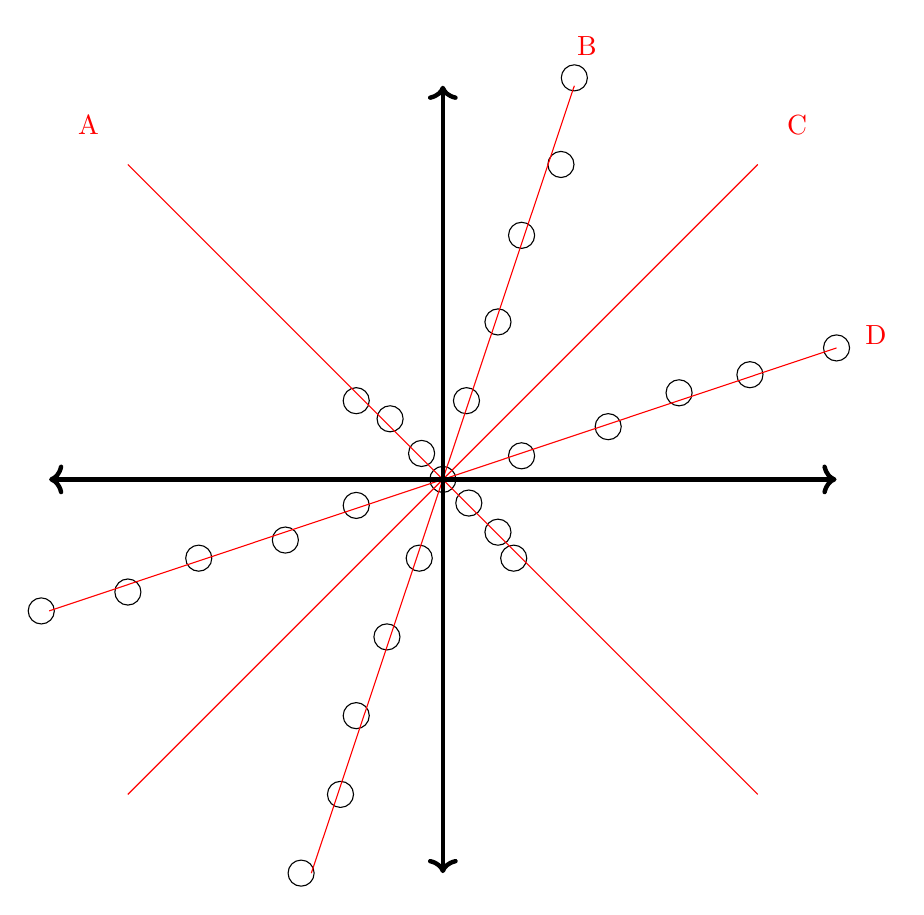
\begin{tikzpicture}
    \begin{scope}[every node/.style={circle,draw}]
    \node (O) at (0,0) {};
    \node (D2) at (1,0.30) {};
    \node (D3) at (2.1, 0.67) {};
    \node (D4) at (3,1.1) {};
    \node (D5) at (3.9,1.33) {};
    \node (D6) at (5,1.67) {};
    \node (D7) at (-1.1,-0.33) {};
    \node (D8) at (-2,-0.77) {};
    \node (D9) at (-3.1,-1.0) {};
    \node (D10) at (-4,-1.43) {};
    \node (D11) at (-5.1,-1.67) {};
    
    \node (B2) at (0.30,1) {};
    \node (B3) at (0.70,2) {};
    \node (B4) at (1.0,3.1) {};
    \node (B5) at (1.5,4) {};
    \node (B6) at (1.67,5.1) {};
    \node (B7) at (-0.30,-1) {};
    \node (B8) at (-0.71,-2) {};
    \node (B9) at (-1.1,-3) {};
    \node (B10) at (-1.30,-4) {};
    \node (B11) at (-1.80,-5) {};
    
    \node (A1) at (-.27, 0.33) {};
    \node (A2) at (-.67, 0.77) {};
    \node (A3) at (-1.1, 1.0) {};
    \node (A4) at (0.33, -0.30) {};
    \node (A5) at (0.70, -0.67) {};
    \node (A6) at (.90, -1.00) {};
    \end{scope}
    
    \draw[red] (-4, -4)--(4, 4);
    \draw[red] (-1.67, -5)--(1.67, 5);
    \draw[red] (-5, -1.67)--(5, 1.67);
    \draw[red] (-4, 4)--(4, -4);
    
    \node[red] (A) at (-4.5, 4.5) {A};
    \node[red] (C) at (4.5, 4.5) {C};
    \node[red] (B) at (1.83, 5.5) {B};
    \node[red] (D) at (5.5, 1.83) {D};

    
    \draw[<->,ultra thick] (-5,0)--(5,0);
    \draw[<->,ultra thick] (0, -5)--(0, 5); 
    \end{tikzpicture}
    \end{figure}
    \end{minipage}
    
\clearpage

    \fullwidth{\textbf{{\large PCA in Practice}}}
    
    \uplevel{
    For this section, refer to the PCA demo linked \href{https://colab.research.google.com/drive/1KF2pVCqQuQABJz_tlSNu1WeHkboV7YG_?usp=sharing}{here}. In this demonstration, we have performed PCA for you on a \href{https://en.wikipedia.org/wiki/Iris_flower_data_set}{simple four-feature dataset}. The questions below have also been added to the colab notebook linked for ease of access. Run the code in the notebook, then answer the questions based on the results.
    }
    
    \part[1] Do you see any special relationships between any of the features? In particular, take a look at the \texttt{petal\_length} feature. How would you describe its association with each of the \textbf{other features}? Select the correct statement with appropriate justification.

    \sone
    \begin{checkboxes}
    % YOUR ANSWER
    % Change \choice to \CorrectChoice for the appropriate selection/selections
    \choice The features are highly correlated: we observe linearly proportional relationships where increases in \verb|petal_length| often correspond to increases in another feature
    \choice The features are highly correlated: we observe that the color classes can be separated with decision boundaries along the \verb|petal_length| axis.
    \choice The features are uncorrelated: we observe random noise as if the features were generated from independent distributions
    \choice The features are uncorrelated: we observe the ``default $y=x$'' relationship between features
    \end{checkboxes}
        
    
    \part[2]  To get the principal components of the features, we calculate the eigenvectors of the covariance matrix, which are orthogonal, along with their corresponding eigenvalues. Which of the following are consequences of the principal components being orthogonal to each other?

    \sall
    {\checkboxchar{$\Box$} \checkedchar{$\blacksquare$}
    \begin{checkboxes}
    % YOUR ANSWER
    % Change \choice to \CorrectChoice for the appropriate selection/selections
    \choice The variance of the data is maximized.
    \choice The reconstruction error is minimized.
    \choice The dot product of any two principal components will be 1.0.
    \choice We can attribute certain variations in the data to unique principal components.
    \choice In the dimensionality-reduced space, the covariance of the first and second dimensions will always be zero.
    \choice It ensures that our lower-dimensional data will be linearly separable.
    \choice None of the above.
    \end{checkboxes}
    }
    
    
    \part[1]  If we wanted to find $k$ principal components such that we preserve \textbf{at least} 95\% of the variance in the data, what would be the value of $k$? Hint: it is helpful here to look at the cumulative variance in the first $k$ components, which we have calculated for you.
    
    \begin{your_solution}[height=2cm, width=.15\textwidth, title=$k$]
    \end{your_solution}
    
\clearpage

    \part[1] If we wanted to perform dimensionality reduction to have just two features, we could pick any two features from the dataset and train a classifier on just those. What is one reason we could prefer the PCA features to just choosing two of the original features to represent our data?
    
    \begin{your_solution}[height=3cm, width=\textwidth]
    \end{your_solution}
    
\end{parts}\clearpage
\sectionquestion{K-Means}
\label{sec:kmeans}

\begin{parts}
\part Consider the 3 datasets A, B and C. Each dataset is classified into $k$ clusters, with centers marked $X$ and cluster membership represented by different colors in the figure. For each dataset, exactly one clustering was generated by K-means with Euclidean distance. Select the image with clusters generated by K-means.

\begin{subparts}
\subpart[1] Dataset A

\begin{minipage}{.2\textwidth}
    \sone
    
    \begin{checkboxes}
    % YOUR ANSWER
    % Change \choice to \CorrectChoice for the appropriate selection/selections
    \choice A.1
    \choice A.2
    \end{checkboxes}
\end{minipage}
\begin{minipage}{.75\textwidth}
\includegraphics[width=.9\linewidth]{figures/d12.png}
\end{minipage}

\subpart[1] Dataset B


\begin{minipage}{.2\textwidth}
    \sone
    
    \begin{checkboxes}
    % YOUR ANSWER
    % Change \choice to \CorrectChoice for the appropriate selection/selections
    \choice B.1
    \choice B.2
    \end{checkboxes}
\end{minipage}
\begin{minipage}{.75\textwidth}
\includegraphics[width=.9\linewidth]{figures/d23.png}
\end{minipage}

\subpart[1] Dataset C

\begin{minipage}{.2\textwidth}
    \sone
    
    \begin{checkboxes}
    % YOUR ANSWER
    % Change \choice to \CorrectChoice for the appropriate selection/selections
    \choice C.1
    \choice C.2
    \end{checkboxes}
\end{minipage}
\begin{minipage}{.75\textwidth}
\includegraphics[width=.9\linewidth]{figures/d32.png}
\end{minipage}

\end{subparts}

\clearpage

 \part Consider a dataset $\mathcal{D}$ with 5 points as shown below. Perform a K-means clustering on this dataset with $k=2$ using the Euclidean distance as the distance function.
 Remember that in the K-means algorithm, one iteration consists of following two steps: first, we assign each data point to its nearest cluster center; second, we recompute each center as the average of the data points assigned to it. Initially, the 2 cluster centers are chosen randomly as $\mu_0$ = (5.3, 3.5), $\mu_1$ = (5.1, 4.2). Parts (a) through (d) refer only to the first iteration of K-means clustering performed on $\mathcal{D}$.
 
\[
\mathcal{D}=\begin{bmatrix}
5.5&3.1\\
5.1&4.8\\
6.6&3.0\\
5.5&4.6\\
6.8&3.8\\
\end{bmatrix}
\]

    \begin{subparts}
    \subpart[1]  Which of the following points will be the new center for cluster 0?
    
    \sone
    \begin{checkboxes}
    % YOUR ANSWER
    % Change \choice to \CorrectChoice for the appropriate selection/selections
    \choice (5.7 , 4.1)
    \choice (5.6 , 4.8)
    \choice (6.3 , 3.3)
    \choice (6.7 , 3.4)
    \end{checkboxes}

    \subpart[1]  Which of the following points will be the new center for cluster 1?
    
    \sone
    \begin{checkboxes}
    % YOUR ANSWER
    % Change \choice to \CorrectChoice for the appropriate selection/selections
    \choice (6.1 , 3.8)
    \choice (5.5 , 4.6)
    \choice (5.4 , 4.7)
    \choice (5.3 , 4.7)
    \end{checkboxes}

    
    \subpart[1]  How many points will belong to cluster 0, using the new centers?
    
    
    \begin{your_solution}[title=Answer, height=2cm, width=3cm]
    \end{your_solution}


    
    \subpart[1]  How many points will belong to cluster 1, using the new centers?
    
    
    \begin{your_solution}[title=Answer, height=2cm, width=3cm]
    \end{your_solution}
    


   \end{subparts}
   
   \part Recall that in K-means clustering we attempt to find $k$ cluster centers $\cv_1 ,\dots ,\cv_k$ such that the total distance between each point and the nearest cluster center is minimized. We thus solve
   $$ \argmin_{\cv_1 ,\dots ,\cv_k} \sum_{i=1}^N \min_{j\in\{1,\dots ,k\}} \|\xv^{(i)} - \cv_j\|_2^2 $$
   where $n$ is the number of data points. Instead of holding the number of clusters $k$ fixed, your friend John tries to also minimize the objective over $k$, solving 
   $$ \argmin_k \argmin_{\cv_1 ,\dots ,\cv_k} \sum_{i=1}^N \min_{j\in\{1,\dots ,k\}} \|\xv^{(i)} - \cv_j\|_2^2 $$

   You found this idea to be a bad one. 

    \begin{subparts}
    \subpart[1]  What is the minimum possible value of the objective function when minimizing over $k$?

    \begin{your_solution}[title=Answer, height=2cm, width=3cm]
    \end{your_solution}
    
    
    \subpart[1]  What is a value of $k$ for which we achieve the minimum possible value of the objective function when $N=100$?

    \begin{your_solution}[title=Answer, height=2cm, width=3cm]
    \end{your_solution}
    \end{subparts}
    
\clearpage

    \part  Consider the following brute-force algorithm for minimizing the K-means objective: Iterate through each possible assignment of the points to $k$ clusters, $\zv = [z^{(1)}, \ldots, z^{(N)}]$. For each assignment $\zv \in \{1,\ldots,k\}^N$, you evaluate the following objective function:
    $$J(\zv) = \argmin_{\cv_1, \ldots, \cv_k} \sum_{i=1}^N ||\xv^{(i)} - \cv_{z^{(i)}} ||_2^2$$
    At the end, you pick the assignment $\zv$ that had lowest $J(\zv)$.
    
    \begin{subparts}
    \subpart[1] Suppose we have $N$ points and $k$ clusters. For how many possible assignments $\zv$ does the brute force algorithm have to evaluate $J(\zv)$?
    
   \begin{your_solution}[title=Answer, height=2cm, width=3cm]
    \end{your_solution}


    \subpart[1] Suppose $N=1000$, $k=10$, and it takes us $0.01$ seconds to evaluate $J(\zv)$ for a single assignment $\zv$. How many seconds will the brute force algorithm take to check all assignments?
    
   \begin{your_solution}[title=Answer, height=2cm, width=3cm]
    \end{your_solution}
    \end{subparts}

    \clearpage
    
    \part Initializing the centers has a big impact on the performance of the K-means clustering algorithm. Usually, we randomly initialize $k$ cluster centers. However, there are other methods, namely, furthest point initialization and $k$-means++ initialization.
    
    \begin{subparts}
    \subpart[1] 
     Is the clustering at convergence generated by furthest point initialization sensitive to outliers? Explain why or why not.
    
    \begin{your_solution}[height=3cm, width=.95\textwidth]
    \end{your_solution}
    
    \begin{figure}[H]
        \centering
        \includegraphics[width=0.5\linewidth]{figures/kmeans.png}
        \caption{2D Dataset}
        \label{fig:KMeans2}
    \end{figure}
    
    
    \subpart[1] 
    
    Explain in 1– 2 sentences why using  $k$-means++ initialization is more likely to choose one sample from each cluster than random initialization when using the dataset in Figure \ref{fig:KMeans2} above.
    
    \begin{your_solution}[height=3cm, width=.95\textwidth]
    \end{your_solution}

    

    \end{subparts}

\end{parts}
\clearpage
\sectionquestion{Ensemble Methods}
\label{sec:ensemble}

\begin{parts}

\part
In the following question, we will explore two different kinds of ensemble methods: the halving algorithm and the doubling algorithm.

\begin{subparts}
\uplevel{Consider the \textbf{halving algorithm}:\\
We first maintain a list of $n$ weak classifiers $h_1, ..., h_n$ which have not yet made mistakes. The training labels and classifier predictions are in $\{-1, 1\}$. For each training sample $(x,y)$, we make prediction based on the majority vote of weak classifiers $\hat{y} = \text{sign} (\sum_{i = 1}^n h_i(x))$. If the majority vote prediction does not equal to the label, we will eliminate all the $h_i$ such that $h_i(x) \neq y$. The final aggregated classifier will be the ensemble of all the remaining classifiers.
}
\subpart[1]
Assume there are a total of $n$ classifiers initially, and at least one classifier left in the end. What would be the big-O bound of the total number of mistakes made in terms of $n$?

\begin{your_solution}[height=2.5cm, width=4cm]
 %YOUR ANSWER
\end{your_solution}



\subpart[1] 
\textbf{Fill in the blank:} We can set the multiplicative penalty $\beta = \rule{1cm}{0.15mm}$ from the weighted majority algorithm to have the weighted majority algorithm be equivalent to the halving algorithm.

 \begin{your_solution}[height=2.5cm, width=4cm]
    \end{your_solution}
    
\subpart[1] 
What weak classifiers are guaranteed to be kept by the halving algorithm? (In one short sentence.)

 \begin{your_solution}[height=3cm, width=.95\textwidth]
    \end{your_solution}

\clearpage

\uplevel{Now we consider another algorithm, the \textbf{doubling algorithm}, which doubles the count of correct classifiers (by making identical copies of the correct classifiers each iteration) when the majority vote is incorrect. }

\subpart[1]
How could we modify the weighted majority algorithm to behave equivalently to the doubling algorithm for every input $x$ and true label $y$?

    \sall
    {\checkboxchar{$\Box$} \checkedchar{$\blacksquare$}
    \begin{checkboxes}
    % YOUR ANSWER
    % Change \choice to \CorrectChoice for the appropriate selection/selections
    \choice Set the factor $\beta = 2$, and perform weight update of all classifiers $h_i$ for which $h_i(x) \neq y$ when the majority vote is incorrect. 
    \choice Set the factor $\beta = \frac{1}{2}$, and perform weight update of all classifiers $h_i$ for which $h_i(x) \neq y$ when the majority vote is correct.
    \choice Set the factor $\beta = \frac{1}{2}$, and perform weight update of all classifiers $h_i$ for which $h_i(x) \neq y$ when the majority vote is incorrect.
    \choice Set the factor $\beta = 2$, and perform weight update of all classifiers $h_i$ for which $h_i(x) = y$ when the majority vote is correct.
    \choice Set the factor $\beta = 2$, and perform weight update of all classifiers $h_i$ for which $h_i(x) = y$ when the majority vote is incorrect.
    \choice None of the above.
    \end{checkboxes}}
\end{subparts}


\part[1] Which of the following is true? \sall
        {%
        \checkboxchar{$\Box$} \checkedchar{$\blacksquare$} % change checkbox style locally
        \begin{checkboxes}
        % YOUR ANSWER
        % Change \choice to \CorrectChoice for the appropriate selection/selections
        \choice In the weighted majority algorithm, the weights associated with the weak learners are learned during training.
        \choice In the AdaBoost algorithm, the weights associated with the weak learners are learned during training.
        \choice In the weighted majority algorithm, the weak learners are learned during training.
        \choice In the AdaBoost algorithm, the weak learners are learned during training.
        \end{checkboxes}
        }

    
\part[1]  \tf Consider some training point $(x^{(i)}, y^{(i)})$ to the AdaBoost algorithm. If for all $t$, the weak learner $h_t$ learned during training at time $t$ correctly classifies $h_t(x^{(i)}) = y^{(i)}$, there will eventually be a finite time $t$ such that the weight assigned to $x^{(i)}$ in the training distribution $\D_t$ reaches exactly $0$.

    \sone
    \begin{checkboxes}
    % YOUR ANSWER
    % Change \choice to \CorrectChoice for the appropriate selection/selections
    \choice True
    \choice False
    \end{checkboxes}

\part[1]  \tf If AdaBoost reaches perfect training accuracy, all weak learners created in subsequent iterations will be identical (i.e., they will produce the same output on any input). Assume we are using deterministically selected weak learners.

    \sone
    \begin{checkboxes}
    % YOUR ANSWER
    % Change \choice to \CorrectChoice for the appropriate selection/selections
    \choice True
    \choice False
    \end{checkboxes}

\part In the following question, we will examine the generalization error of AdaBoost using a concept known as the \textit{classification margin}.

Throughout the question, use the following definitions:
\begin{itemize}
    \item $N$: The number of training samples.
    \item $S = \{(x^{(1)}, y^{(1)}), \cdots, (x^{(N)}, y^{(N)})\}$: The training samples with binary labels ($y^{(i)} \in \{-1, +1\}$).
    \item $\D_t (i)$: The weight assigned to training example $i$ at time $t$. Note that $\sum_i \D_t (i) = 1$.
    \item $h_t$: The weak learner constructed at time $t$.
    \item $\epsilon_t$: The error of $h_t$ on $\D_t$.
    \item $Z_t$: The normalization factor for the distribution update at time $t$.
    \item $\alpha_t$: The weight assigned to the learner $h_t$ in the composite hypothesis.
    \item $f_t (x) = \left( \sum_{t'=1}^{t} \alpha_{t'} h_{t'} (x) \right) / \left( \sum_{t'=1}^{t} \alpha_{t'} \right)$: The aggregated vote of the weak learners, rescaled based on the total weight.
\end{itemize}

For a binary classification task, assume that we use a probabilistic classifier that provides a probability distribution over the possible labels (i.e. $p(y|x)$ for $y \in \{+1,-1\}$). The classifier output is the label with highest probability.
We define the \textit{classification margin} for an input as the signed difference between the probability assigned to the correct label and the incorrect label $p_{correct} - p_{incorrect}$, which takes on values in the range $[-1, 1]$.
Recall from recitation that $\margin_t (x^{(i)}, y^{(i)}) = y^{(i)} f_t (x^{(i)})$.

\begin{subparts}
\subpart[1]  Recall the update AdaBoost performs on the distribution of weights:
\begin{itemize}
    \item $\D_1 (i) = 1 / N$
    \item $\D_{t+1} (i) = \D_t (i) \dfrac{\exp(-y^{(i)} \alpha_t h_t (x^{(i)}))}{Z_t} = \dfrac{1}{N} \left( \prod_{t'=1}^t \dfrac{1}{Z_{t'}} \right) \exp ( - \sum_{t'=1}^t y^{(i)} \alpha_{t'} h_{t'} (x^{(i)}) )$
\end{itemize}
We define $C_{t+1} = \dfrac{1}{N} \left( \prod_{t'=1}^t \dfrac{1}{Z_{t'}} \right)$ and $M_{t+1} (i) =  -\sum_{t'=1}^t y^{(i)} \alpha_{t'} h_{t'} (x^{(i)})$. 
We then have $$\D_{t+1} (i) = C_{t+1} \exp (M_{t+1} (i))$$

Let $\alpha = \sum_{t'=1}^t \alpha_{t'}$. Rewrite $M_{t+1} (i)$ in terms of $\margin_t (x^{(i)}, y^{(i)})$ and $\alpha$. (Hint: first rewrite $M_{t+1} (i)$ in terms of $y^{(i)}, \alpha, f_t, x^{(i)}$, then apply our given formula for the margin).

\begin{your_solution}[height=2.5cm, width=6cm]
\end{your_solution}

\clearpage

\subpart[1]  Note that $C_{t+1}, \alpha$ are treated as positive constants with respect to the input points. Using the classification margin and the above formulation of the weights assigned by AdaBoost, fill in the blanks to describe which points AdaBoost assigns high weight to at time $t$.

At time $t$, AdaBoost assigns higher weight to points $x^{(i)}$ with \rule{1cm}{0.15mm} \rule{1cm}{0.15mm} value of margin on the current ensemble classifier (i.e., $\margin_t (x^{(i)}, y^{(i)})$).

    \sone
    \begin{checkboxes}
    % YOUR ANSWER
    % Change \choice to \CorrectChoice for the appropriate selection/selections
    \choice higher absolute
    \choice higher signed
    \choice lower absolute
    \choice lower signed
    \end{checkboxes}

\subpart[1] How does this weighting behavior explain the empirical result of test error continuing to decrease after training error has converged?

 \begin{your_solution}[height=3cm, width=.95\textwidth]
    \end{your_solution}

\end{subparts}

\end{parts}


\clearpage
\sectionquestion{Recommender Systems}
\label{sec:recsys}

\begin{parts}

 \part[2]  In which of the following situations will a collaborative filtering system be a more appropriate learning algorithm than a linear or logistic regression model?
    
    \sall
    {\checkboxchar{$\Box$} \checkedchar{$\blacksquare$}
        \begin{checkboxes}
        % YOUR ANSWER
        % Change \choice to \CorrectChoice for the appropriate selection/selections 
        \choice You manage an online bookstore, and you have book ratings and sales data from many users. For each user, you want to recommend other books she will enjoy, based on her own ratings and the ratings of other users.
        \choice You manage an online bookstore, and you have book ratings and sales data from many users. You want to learn to predict the expected sales volume (number of books sold) as a function of the average rating of a book.
        \choice You run an online news aggregator, and for every user, you know some subset of articles that the user likes and some different subset that the user dislikes. You want to use this to find other articles that the user likes.
        \choice You've written a piece of software that downloads news articles from many news websites. In your system, you also keep track of which articles you personally like and which ones you dislike, and the system also stores away features of these articles (e.g., word counts, name of author). Using this information, you want to build a system to try to find additional new articles that you personally will like.
        \choice None of the above
        \end{checkboxes}
    }

 

 \part[2]  What is the basic intuition behind matrix factorization?
    
    \sall
    {\checkboxchar{$\Box$} \checkedchar{$\blacksquare$}
        \begin{checkboxes}
        % YOUR ANSWER
        % Change \choice to \CorrectChoice for the appropriate selection/selections 
        \choice That content filtering and collaborative filtering are just two different factorizations of the same rating matrix.
        \choice That factoring user and item matrices can partition the users and items into clusters that can be treated identically, reducing the complexity of making recommendations.
        \choice The user-user and item-item correlations are more efficiently computed by factoring matrices, even when including the cost of factoring matrices.
        \choice That users and items can be well described in a shared low dimensional space that can be computed from the rating matrices.
        \choice None of the above
        \end{checkboxes}
    }
    
    
    
\part Neural the Narwhal decides to set up a friend-recommendation system for all the students in 10-301/601, of which there are $N = 10,301,601$. Ideally, Neural would store the full $N \times N$ matrix $M$, where $M_{ij}$ is 1 if student $i$ and $j$ are friends and 0 if student $i$ and $j$ are nemeses, or \texttt{null} if students $i$ and $j$ have never met. Assume that these are the only possible relationships between 2 people and that all relationships are symmetric (so it cannot be the case that student $i$ thinks student $j$ is their friend while $j$ thinks $i$ is their nemesis). Unfortunately, storing $M$ in its entirety would take over 10 TB of storage, which Neural cannot afford on a TA salary. Neural instead uses the following procedure to approximate $M$ as $U U^T$ for some low rank $N \times d$ matrix $U$, where each row of $U$ corresponds to a student.

\algrenewcommand{\algorithmiccomment}[1]{\hfill// #1}
\algtext*{EndWhile}% Remove "end while" text
\algtext*{EndIf}% Remove "end if" text
\begin{algorithm}
\begin{algorithmic}[1]
\State Given learning rate $\eta$, ground truth relationships $M$
\State Randomly initialize user embedding matrix $U \in \mathbb{R}^{N \times d}$

\While{not converged}
    \State Sample $i \sim$ Uniform(1, $N$), $j \sim$ Uniform(1, $N$)
    \State $\hat{M}_{ij} \gets \sigma(\vec{u}_i^T \vec{u}_j)$ 
    \Comment{$\sigma$ is sigmoid function}
    \State $\mathcal{L}(\vec{u}_i, \vec{u}_j) \gets -M_{ij} \log(\hat{M}_{ij}) - (1-M_{ij})\log(1 - \hat{M}_{ij})$
    \Comment{Compute logistic loss}
    \State $\vec{g}_i \gets \nabla_{\vec{u}_i} \mathcal{L}(\vec{u}_i, \vec{u}_j)$
    \Comment{Compute and perform gradient updates}
    \State $\vec{g}_j \gets \nabla_{\vec{u}_j} \mathcal{L}(\vec{u}_i, \vec{u}_j)$
    \State $\vec{u}_i$ $\gets$ $\vec{u}_i$ - $\eta \cdot \vec{g}_i$
    \State $\vec{u}_j$ $\gets$ $\vec{u}_j$ - $\eta \cdot \vec{g}_j$
\EndWhile

\end{algorithmic}
\end{algorithm}

\begin{subparts}
\subpart[2] One of the lines in the above algorithm is incorrect. State the line number, and provide the correct line.\\
    \begin{your_solution}[title=Line \#, height=2cm, width=.2\textwidth]
    \end{your_solution}
    \begin{your_solution}[title=Fixed line of code, height=2cm, width=.75\textwidth]
    \end{your_solution}

\subpart[1] Based on the loss function given on line 6, derive an expression for $\nabla_{\vec{u}_j} \mathcal{L}(\vec{u}_i, \vec{u}_j)$ in terms of $\vec{u}_i$, $\vec{u}_j$, and $M_{ij}$. Note that $\sigma$ denotes the sigmoid function and $\log$ is natural log. \\
    \begin{your_solution}[height=3cm, width=.95\textwidth]
    \end{your_solution}
    

\subpart[2] Why is it appropriate here to factorize $M$ as the product of a single matrix by itself $U U^T$ rather than as the product of two distinct matrices $VW^T$?

    \sall
    {\checkboxchar{$\Box$} \checkedchar{$\blacksquare$}
    \begin{checkboxes}
    % YOUR ANSWER
    % Change \choice to \CorrectChoice for the appropriate selection/selections
    \choice $U U^T$ enforces that our approximation is symmetric, while $VW^T$ is not necessarily symmetric.
    \choice SGD is guaranteed to converge faster and to a better optimum for $U$ because we have fewer parameters to learn.
    \choice We can parallelize training for $U$, whereas we could not parallelize training for $V$ and $W$.
    \choice We wish to model relationships between objects of a single type, not between objects of two different types.
    \choice None of the above.
    \end{checkboxes}
    }
    

\end{subparts}

\end{parts}
\end{questions}

\newpage
\newpage
\section{Collaboration Questions}
After you have completed all other components of this assignment, report your answers to these questions regarding the collaboration policy. Details of the policy can be found \href{http://www.cs.cmu.edu/~mgormley/courses/10601/syllabus.html}{here}.
\begin{enumerate}
    \item Did you receive any help whatsoever from anyone in solving this assignment? If so, include full details.
    \item Did you give any help whatsoever to anyone in solving this assignment? If so, include full details.
    \item Did you find or come across code that implements any part of this assignment? If so, include full details.
\end{enumerate}

\begin{your_solution}[height=6cm]
% YOUR ANSWER 

\end{your_solution}

\end{document}